%%%%%%%%%%%%%%%%%%%%%%%%%%%%%%%%%%%%%%%%%
% Wenneker Assignment
% LaTeX Template
% Version 2.0 (12/1/2019)
%
% This template originates from:
% http://www.LaTeXTemplates.com
%
% Authors:
% Vel (vel@LaTeXTemplates.com)
% Frits Wenneker
%
% License:
% CC BY-NC-SA 3.0 (http://creativecommons.org/licenses/by-nc-sa/3.0/)
% 
%%%%%%%%%%%%%%%%%%%%%%%%%%%%%%%%%%%%%%%%%

%----------------------------------------------------------------------------------------
%	PACKAGES AND OTHER DOCUMENT CONFIGURATIONS
%----------------------------------------------------------------------------------------

\documentclass[11pt]{scrartcl} % Font size

%%%%%%%%%%%%%%%%%%%%%%%%%%%%%%%%%%%%%%%%%
% Wenneker Assignment
% Structure Specification File
% Version 2.0 (12/1/2019)
%
% This template originates from:
% http://www.LaTeXTemplates.com
%
% Authors:
% Vel (vel@LaTeXTemplates.com)
% Frits Wenneker
%
% License:
% CC BY-NC-SA 3.0 (http://creativecommons.org/licenses/by-nc-sa/3.0/)
% 
%%%%%%%%%%%%%%%%%%%%%%%%%%%%%%%%%%%%%%%%%

%----------------------------------------------------------------------------------------
%	PACKAGES AND OTHER DOCUMENT CONFIGURATIONS
%----------------------------------------------------------------------------------------

\usepackage{amsmath, amsfonts, amsthm} % Math packages

\usepackage{listings} % Code listings, with syntax highlighting

\usepackage[english]{babel} % English language hyphenation

\usepackage{graphicx} % Required for inserting images
\usepackage{caption}
\graphicspath{{Figures/}{./}} % Specifies where to look for included images (trailing slash required)

\usepackage{booktabs} % Required for better horizontal rules in tables

\numberwithin{equation}{section} % Number equations within sections (i.e. 1.1, 1.2, 2.1, 2.2 instead of 1, 2, 3, 4)
\numberwithin{figure}{section} % Number figures within sections (i.e. 1.1, 1.2, 2.1, 2.2 instead of 1, 2, 3, 4)
\numberwithin{table}{section} % Number tables within sections (i.e. 1.1, 1.2, 2.1, 2.2 instead of 1, 2, 3, 4)

\setlength\parindent{0pt} % Removes all indentation from paragraphs

\usepackage{enumitem} % Required for list customisation
\setlist{noitemsep} % No spacing between list items

%----------------------------------------------------------------------------------------
%	DOCUMENT MARGINS
%----------------------------------------------------------------------------------------

\usepackage{geometry} % Required for adjusting page dimensions and margins

\geometry{
	paper=a4paper, % Paper size, change to letterpaper for US letter size
	top=2.5cm, % Top margin
	bottom=3cm, % Bottom margin
	left=3cm, % Left margin
	right=3cm, % Right margin
	headheight=0.75cm, % Header height
	footskip=1.5cm, % Space from the bottom margin to the baseline of the footer
	headsep=0.75cm, % Space from the top margin to the baseline of the header
	%showframe, % Uncomment to show how the type block is set on the page
}

%----------------------------------------------------------------------------------------
%	FONTS
%----------------------------------------------------------------------------------------

\usepackage[utf8]{inputenc} % Required for inputting international characters
\usepackage[T1]{fontenc} % Use 8-bit encoding

\usepackage{fourier} % Use the Adobe Utopia font for the document

%\usepackage[framed,numbered,autolinebreaks,useliterate]{mcode}

%----------------------------------------------------------------------------------------
%	SECTION TITLES
%----------------------------------------------------------------------------------------

\usepackage{sectsty} % Allows customising section commands

\sectionfont{\normalfont\bfseries} % \section{} styling
\subsectionfont{\normalfont\bfseries} % \subsection{} styling
\subsubsectionfont{\normalfont\itshape} % \subsubsection{} styling
\paragraphfont{\normalfont\scshape} % \paragraph{} styling

%----------------------------------------------------------------------------------------
%	HEADERS AND FOOTERS
%----------------------------------------------------------------------------------------

\usepackage{scrlayer-scrpage} % Required for customising headers and footers

\ohead*{} % Right header
\ihead*{} % Left header
\chead*{} % Centre header

\ofoot*{} % Right footer
\ifoot*{} % Left footer
\cfoot*{\pagemark} % Centre footer

% MY PACKAGES
%\usepackage[framed,numbered,autolinebreaks,useliterate]{mcode}
\usepackage{listings}
\usepackage{float}
\usepackage{amsmath}
\usepackage{tikz}
\usetikzlibrary{shapes,arrows,positioning}
\usepackage{hyperref} % Include the file specifying the document structure and custom commands

%----------------------------------------------------------------------------------------
%	TITLE SECTION
%----------------------------------------------------------------------------------------

\title{	
	\normalfont\normalsize
	\textsc{Universität Würzburg}\\ % Your university, school and/or department name(s)
	\vspace{25pt} % Whitespace
	\rule{\linewidth}{0.5pt}\\ % Thin top horizontal rule
	\vspace{20pt} % Whitespace
	{\huge Übung 8}\\ % The assignment title
	{\Large Beobachter}\\
	\vspace{12pt} % Whitespace
	\rule{\linewidth}{2pt}\\ % Thick bottom horizontal rule
	\vspace{12pt} % Whitespace
}

\author{\LARGE Alexander Björk, Janis Kaltenthaler} % Your name

\date{\normalsize\today} % Today's date (\today) or a custom date

\begin{document}

\maketitle % Print the title

\tikzstyle{block} = [draw, fill=blue!20, rectangle, 
    minimum height=3em, minimum width=6em]
\tikzstyle{sum} = [draw, fill=blue!20, circle, node distance=1cm]
\tikzstyle{input} = [coordinate]
\tikzstyle{output} = [coordinate]
\tikzstyle{pinstyle} = [pin edge={to-,thin,black}]
\newcommand{\inte}{$\displaystyle \int$}

\section*{Aufgabe 8-1. Beobachterentwurf (3 Punkte)}
\subsection*{a)}
Zu prüfen ist ob die Regelstrecke vollständig steuerbar und vollständig beobachtbar ist:
\subsubsection*{Steuerbarkeit}
\begin{align*}
	S_S&=\begin{bmatrix}b&Ab \end{bmatrix}=\begin{bmatrix}0&-0.5\\0.5&-1 \end{bmatrix}\\
	\text{det}\hspace{3pt}S_S&=0.25\neq0
\end{align*}
Die Regelstrecke ist vollständig Steuerbar.
\subsubsection*{Beobachtbarkeit}
\begin{align*}
	S_B&=\begin{bmatrix}C\\CA \end{bmatrix}=\begin{bmatrix}0&1\\1&-2 \end{bmatrix}\\
	\text{det}\hspace{3pt}S_B&=-1\neq0
\end{align*}
Die Regelstrecke ist vollständig beobachtbar.
\subsection*{b)}
Aufgrund der Struktur des gegebenen Zustandsraummodells wissen wir dass dieses in der Beobachtungsnormalform vorliegt.\\
Die geforderten Eigenwerte des Beobachtermodells sind mit $\lambda_{B1}=-4$ und $\lambda_{B2}=-3$ gegeben. Daraus ergibt sich folgendes charakteristisches Polynom:
\begin{align*}
	p(\lambda_B)=\lambda^2+\underbrace{7}_{a_{B1}}\cdot\lambda+\underbrace{12}_{a_{B_0}}
\end{align*}
Die Koeffizienten $a_0=1$ und $a_1=2$ des charakteristischen Polynoms der Regelstrecke erhalten wird durch Ablesen aus dem gegebenen Zustandsraummodells.\\
Wie folgt kann nun die Beobachterrückführung berechnet werden:
\begin{align*}
	l^T=\begin{bmatrix}a_{B0}&a_{B1}\end{bmatrix}-\begin{bmatrix}a_{0}&a_{1}\end{bmatrix}=\begin{bmatrix}11&5\end{bmatrix}
\end{align*}

%Der Luenbergerbeobachter für das gegebene System hat nun die folgende Form:
%\begin{align*}
%	\dot{\hat{x}}(t)&=(A-lc^t)\hat{x}(t)+bu(t)+ly(t)\\
%	\dot{\hat{x}}(t)&=\begin{bmatrix}0&-12\\1&-7\end{bmatrix}\hat{x}(t)+\begin{bmatrix}0\\0.5\end{bmatrix}u(t)+\begin{bmatrix}11\\5\end{bmatrix}y(t)
%\end{align*}
Das Zustandsraummodell der Regelstrecke und des Beobachters erhält man wie folgt:
\begin{align*}
	\dot{\tilde{x}}(t)&=\begin{bmatrix}\dot{x}(t)\\\dot{\hat{x}}(t)\end{bmatrix}=\begin{bmatrix}A&0\\lc^T&A-lc^T\end{bmatrix}\cdot\begin{bmatrix}x(t)\\\hat{x}(t)\end{bmatrix}+\begin{bmatrix}B&E\\B&0\end{bmatrix}\cdot \begin{bmatrix}u(t)\\d(t)\end{bmatrix}\\
	y(t)&=\begin{bmatrix}C&0\end{bmatrix}\cdot\begin{bmatrix}x(t)\\\hat{x}(t)\end{bmatrix}\\\\
	\dot{\tilde{x}}(t)&=\begin{bmatrix}\dot{x}(t)\\\dot{\hat{x}}(t)\end{bmatrix}=\begin{bmatrix}0&-1&0&0\\1&-2&0&0\\0&11&0&-12\\0&5&1&-7\end{bmatrix}\cdot\begin{bmatrix}x(t)\\\hat{x}(t)\end{bmatrix}+\begin{bmatrix}0&0\\0.5&1\\0&0\\0.5&0\end{bmatrix}\cdot \begin{bmatrix}u(t)\\d(t)\end{bmatrix}\\
	y(t)&=\begin{bmatrix}0&1&0&0\end{bmatrix}\cdot\begin{bmatrix}x(t)\\\hat{x}(t)\end{bmatrix}
\end{align*}
\subsection*{c)}
\begin{figure}[H]
\centering
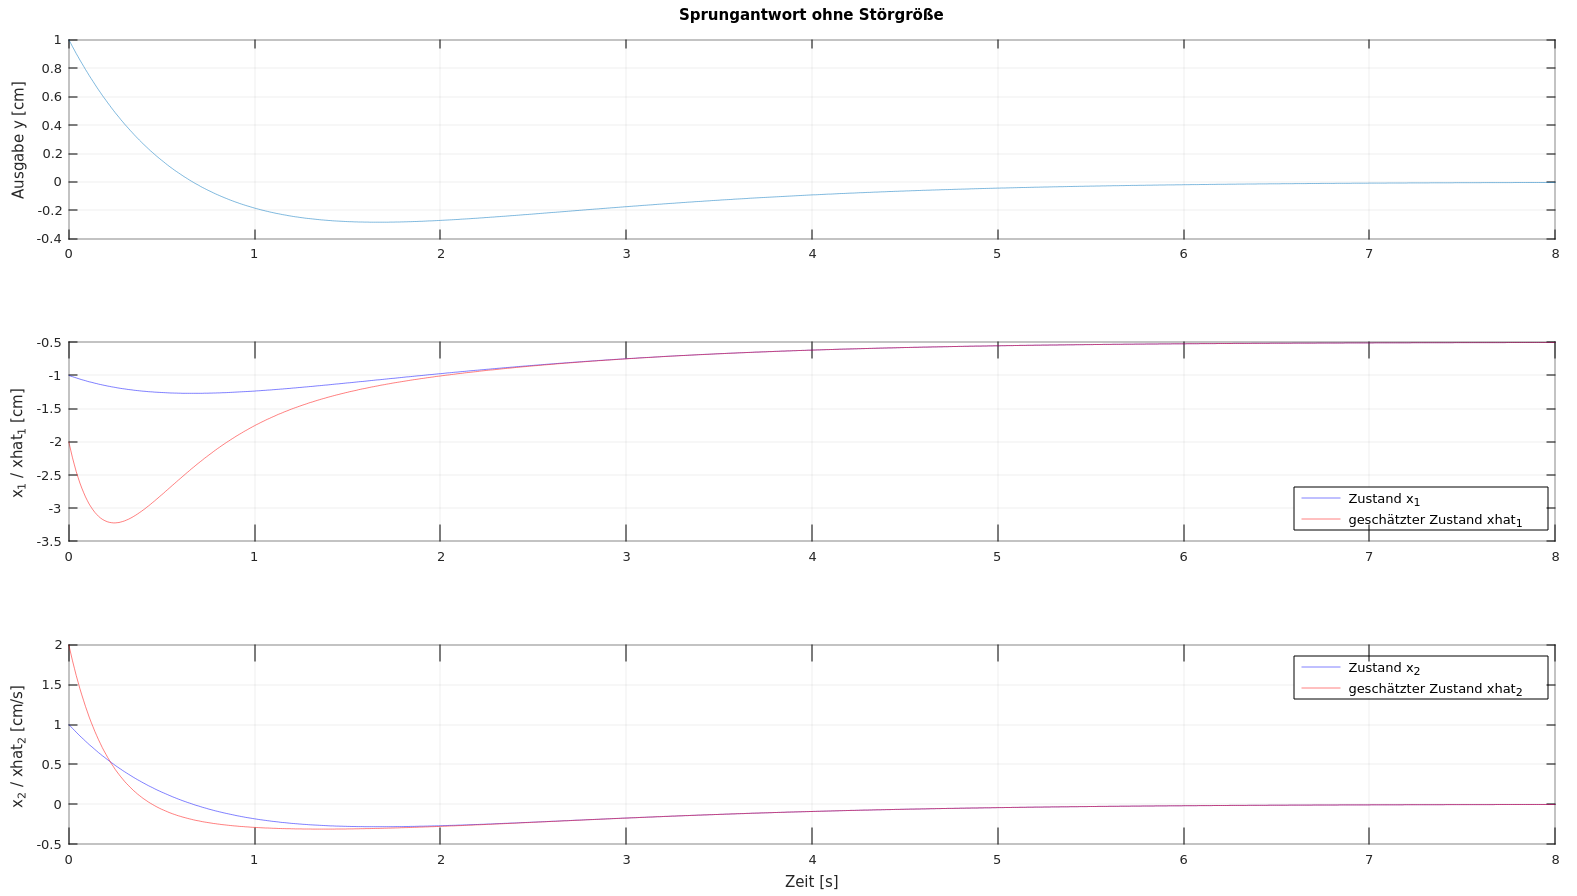
\includegraphics[width=\textwidth]{ohneStoergroesse.png}
\captionsetup{labelformat=empty}
\caption{Abb. 8-1.1: Sprungantwort ohne Störgröße.}
\end{figure}
Etwa zum Zeitpunkt $t=2s$ stimmt der geschätzte Zustand mit dem tatsächlichen Zustand überein.

\subsection*{d)}
\begin{figure}[H]
\centering
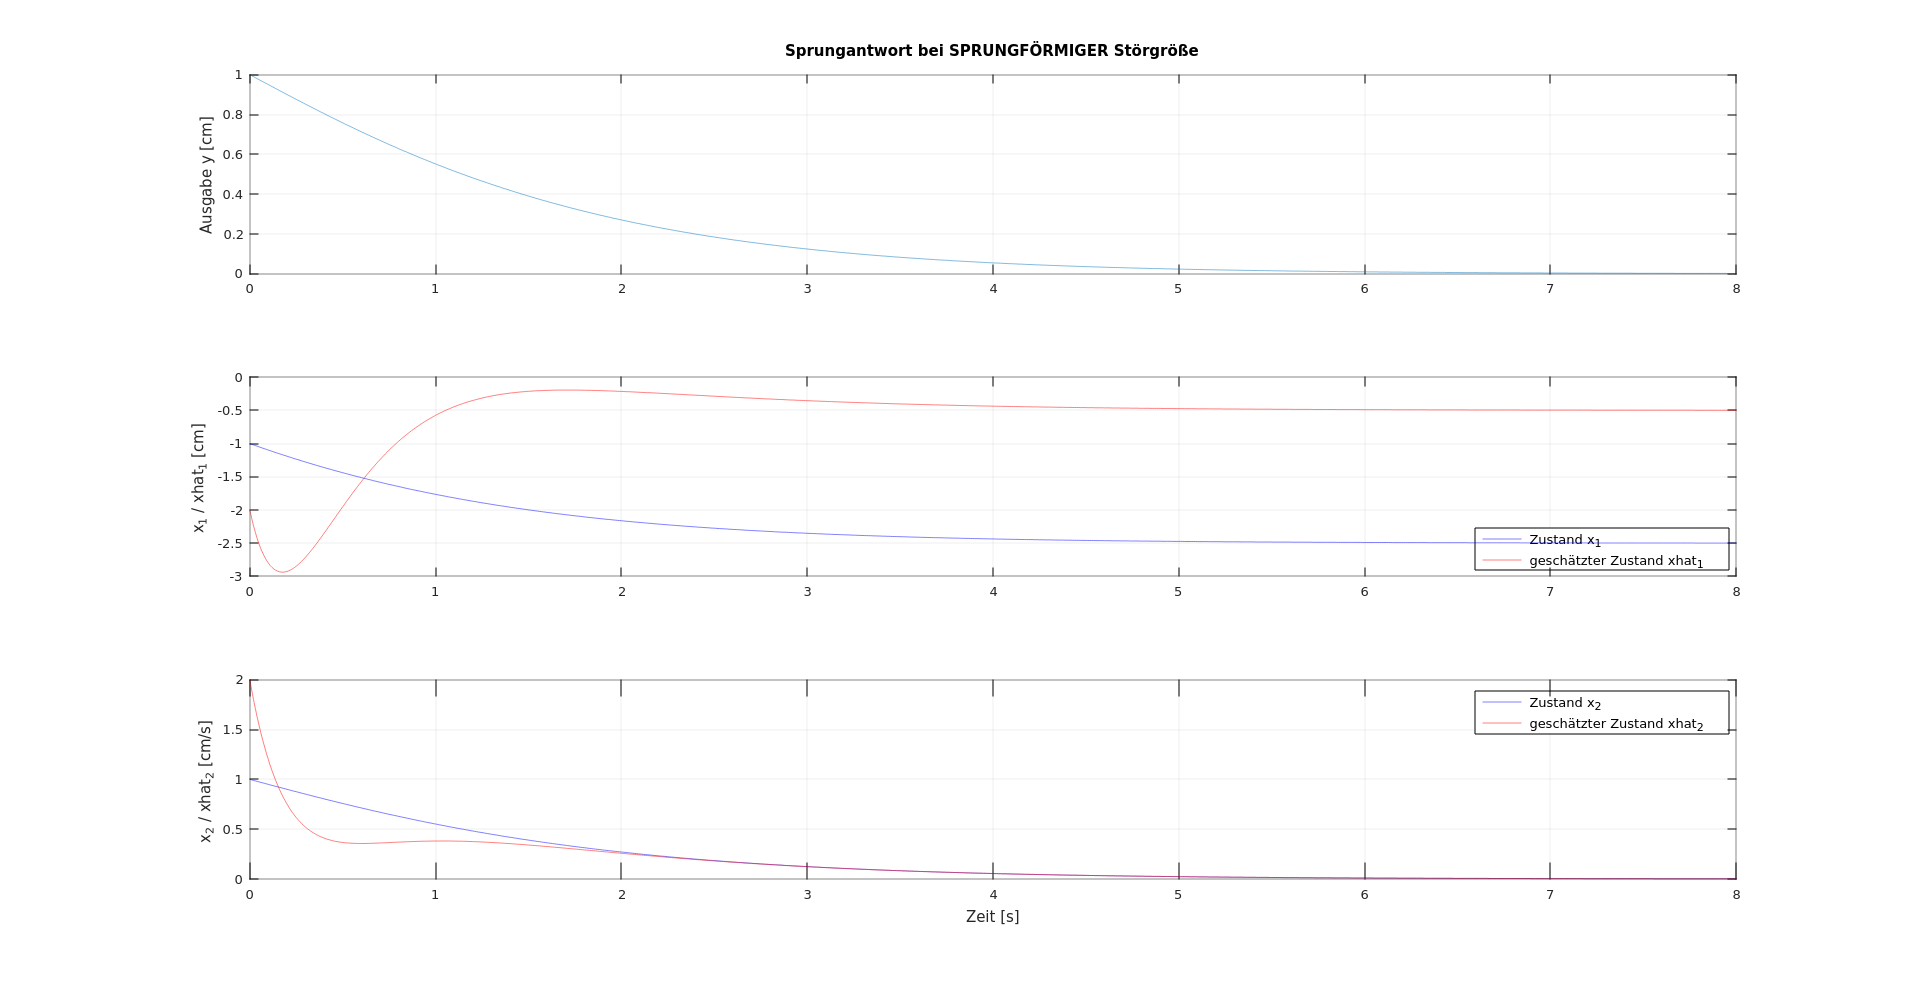
\includegraphics[width=\textwidth]{sprungfoermigeStoergroesse.png}
\captionsetup{labelformat=empty}
\caption{Abb. 8-1.2: Sprungantwort mit sprungförmiger Störgröße.}
\end{figure}

\begin{figure}[H]
\centering
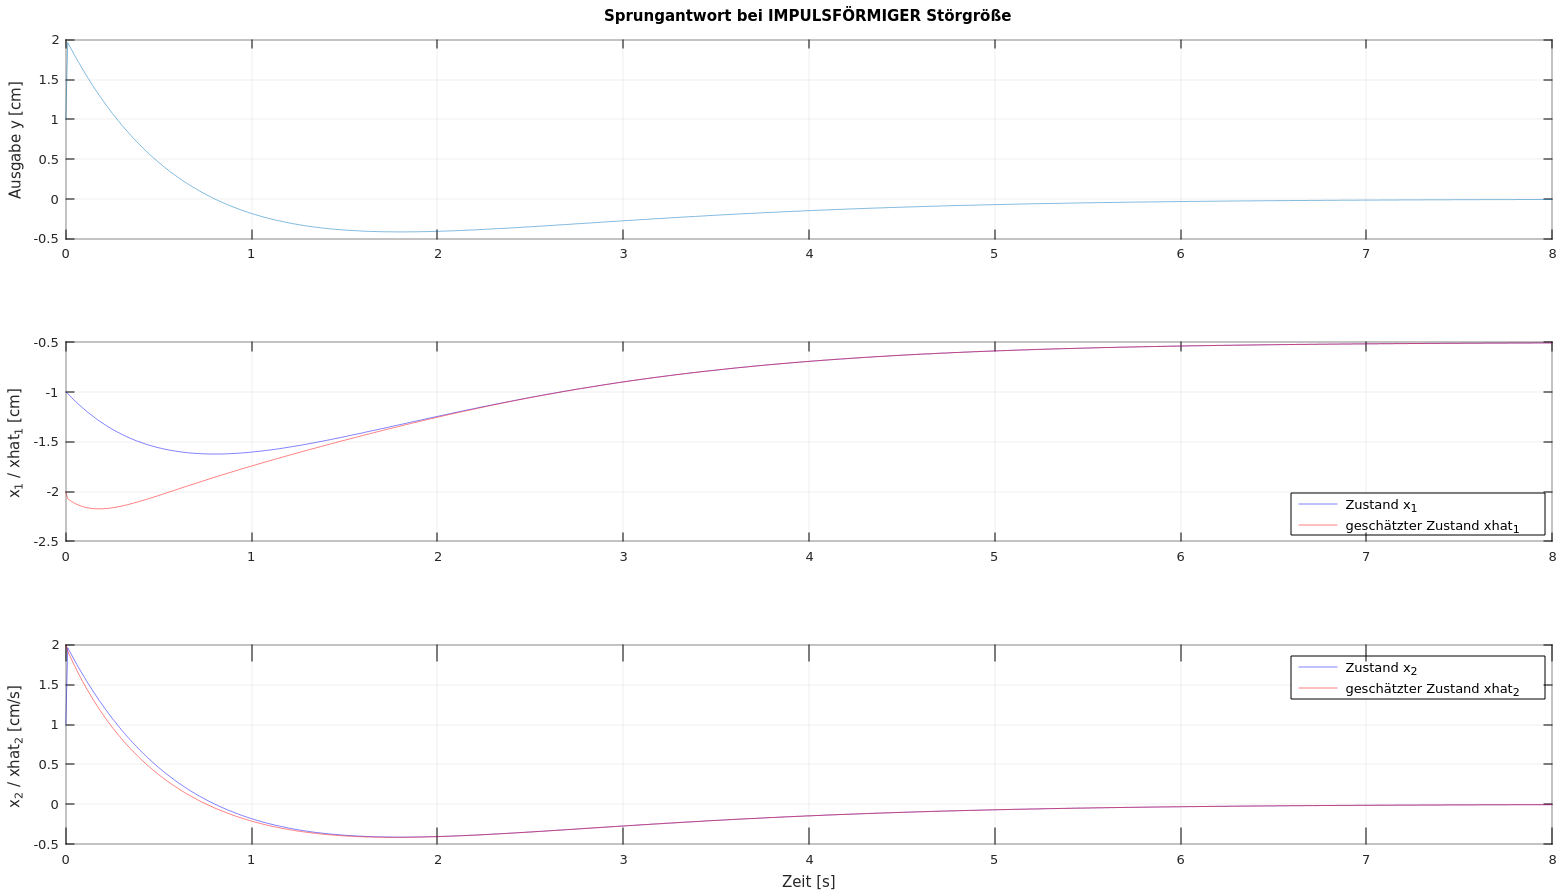
\includegraphics[width=\textwidth]{impulsfoermigeStoergroesse.png}
\captionsetup{labelformat=empty}
\caption{Abb. 8-1.3: Sprungantwort mit impulsförmiger Störgröße.}
\end{figure}

\begin{figure}[H]
\centering
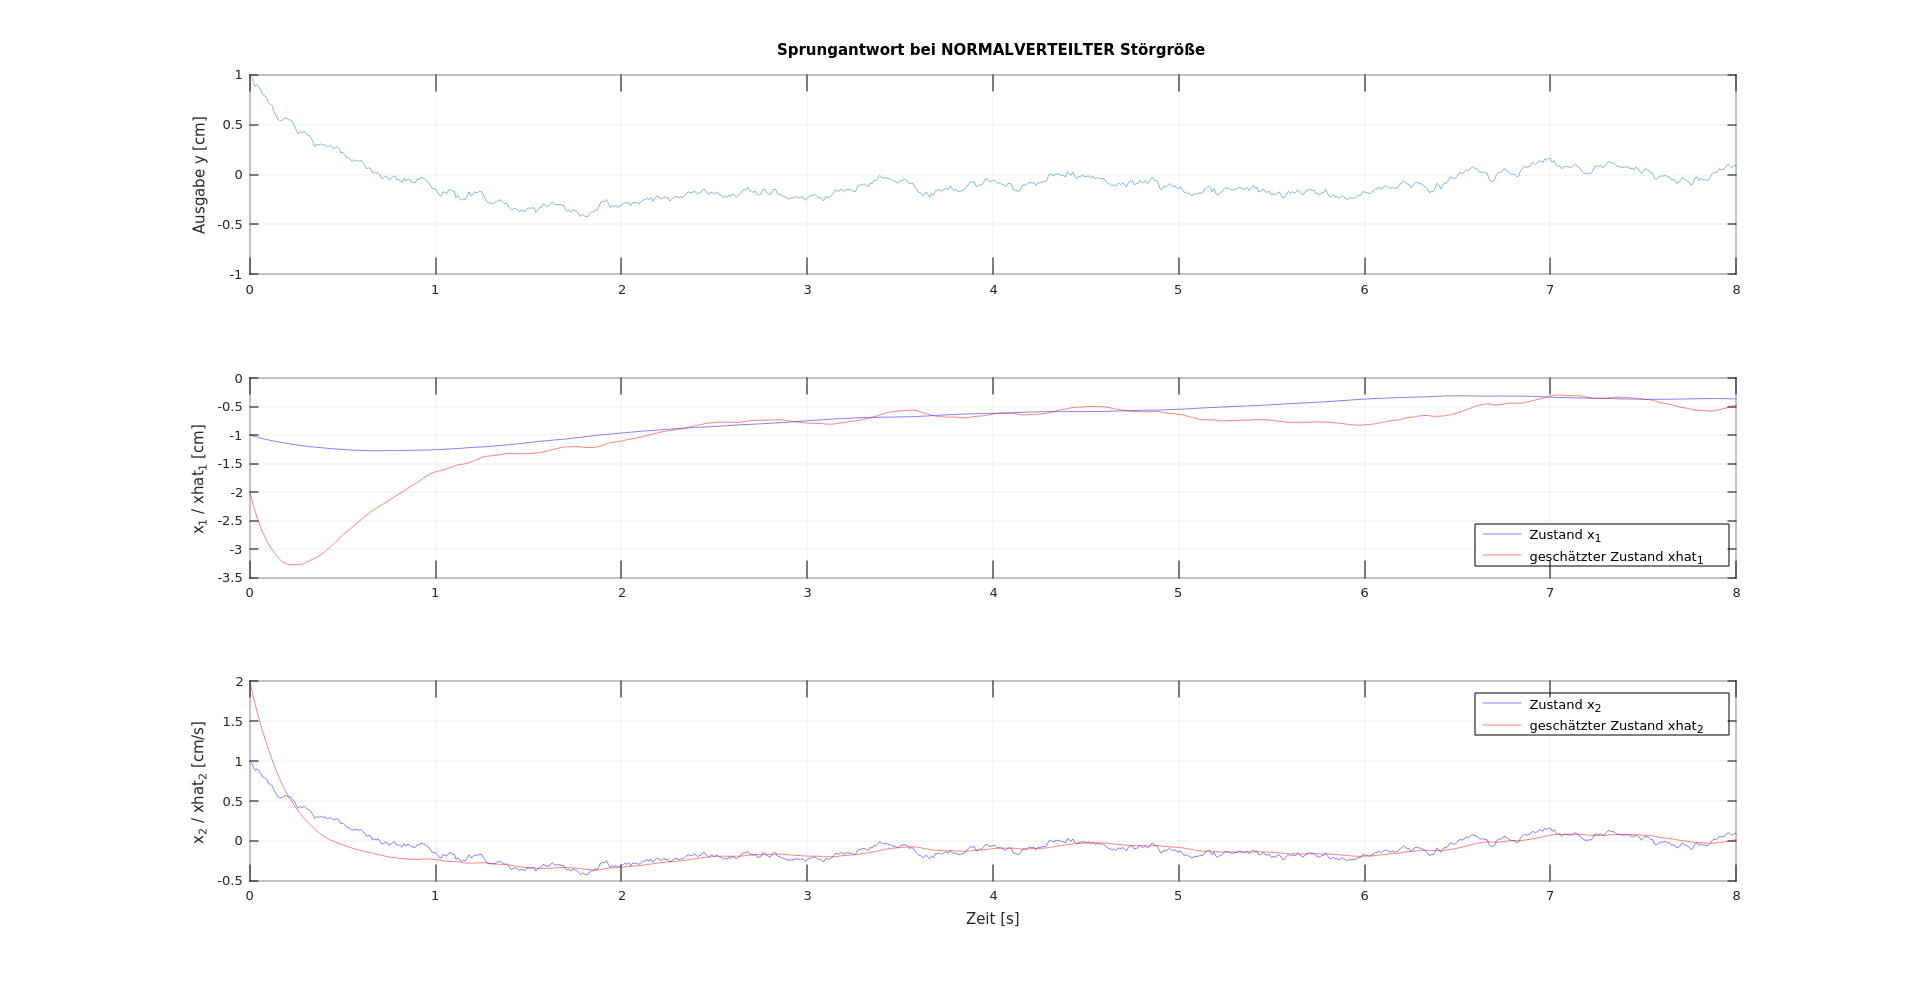
\includegraphics[width=\textwidth]{normalverteilteStoergroesse.png}
\captionsetup{labelformat=empty}
\caption{Abb. 8-1.4: Sprungantwort mit normalverteilter Störgröße.}
\end{figure}

Wirkt eine sprungförmige Störgröße auf die Regelstrecke, so bleibt eine stetige Abweichung zwischen dem geschätzten Zustand der ersten Zustandsvariable und dem tatsächlichen Zustand.\\
Wirkt eine normalverteilte oder impulsförmige Störgröße auf die Regelstrecke, so nähert sich sich der geschätzte Zustand dem tatsächlichen Zustand an.


\section*{Aufgabe 8-2. Beobachterentwurf mit Zustandsrückführung (3 Punkte)}
\subsection*{a)}
Die vollständige Steuerbarkeit und vollständige Beobachtbarkeit wurde mit Matlab geprüft.
\subsection*{b)}
Die Eigenwerte des Beobachters wurden mit $\lambda_{B1}=-9$ und $\lambda_{B2}=-12$ festgelegt.\\
Mithilfe von Matlab wurde das resultierende Zustandsraummodell des geschlossenen Regelkreises mit Beobachter berechnet:
\begin{align*}
	\dot{\tilde{x}}(t)&=\begin{bmatrix}\dot{x}(t)\\\dot{\hat{x}}(t)\end{bmatrix}=\begin{bmatrix}0&1&0&0\\-1&1&-11&-8\\22&0&-22&1\\129&0&-141&-7\end{bmatrix}\cdot\begin{bmatrix}x(t)\\\hat{x}(t)\end{bmatrix}+\begin{bmatrix}0\\12\\0\\12\end{bmatrix}\cdot u(t)\\
	y(t)&=\begin{bmatrix}0&1&0&0\end{bmatrix}\cdot\begin{bmatrix}x(t)\\\hat{x}(t)\end{bmatrix}
\end{align*}
\subsection*{c)}
Für die Simulation wurde eine sprungförmige Stellgröße genutzt. Die Anfangszustände wurden wie folgt gesetzt:
\begin{align*}
	x_0(t)=\begin{bmatrix}-1\\1\end{bmatrix},\hspace{10pt}\hat{x}_0(t)=\begin{bmatrix}-2\\2\end{bmatrix}
\end{align*}
\begin{figure}[H]
\centering
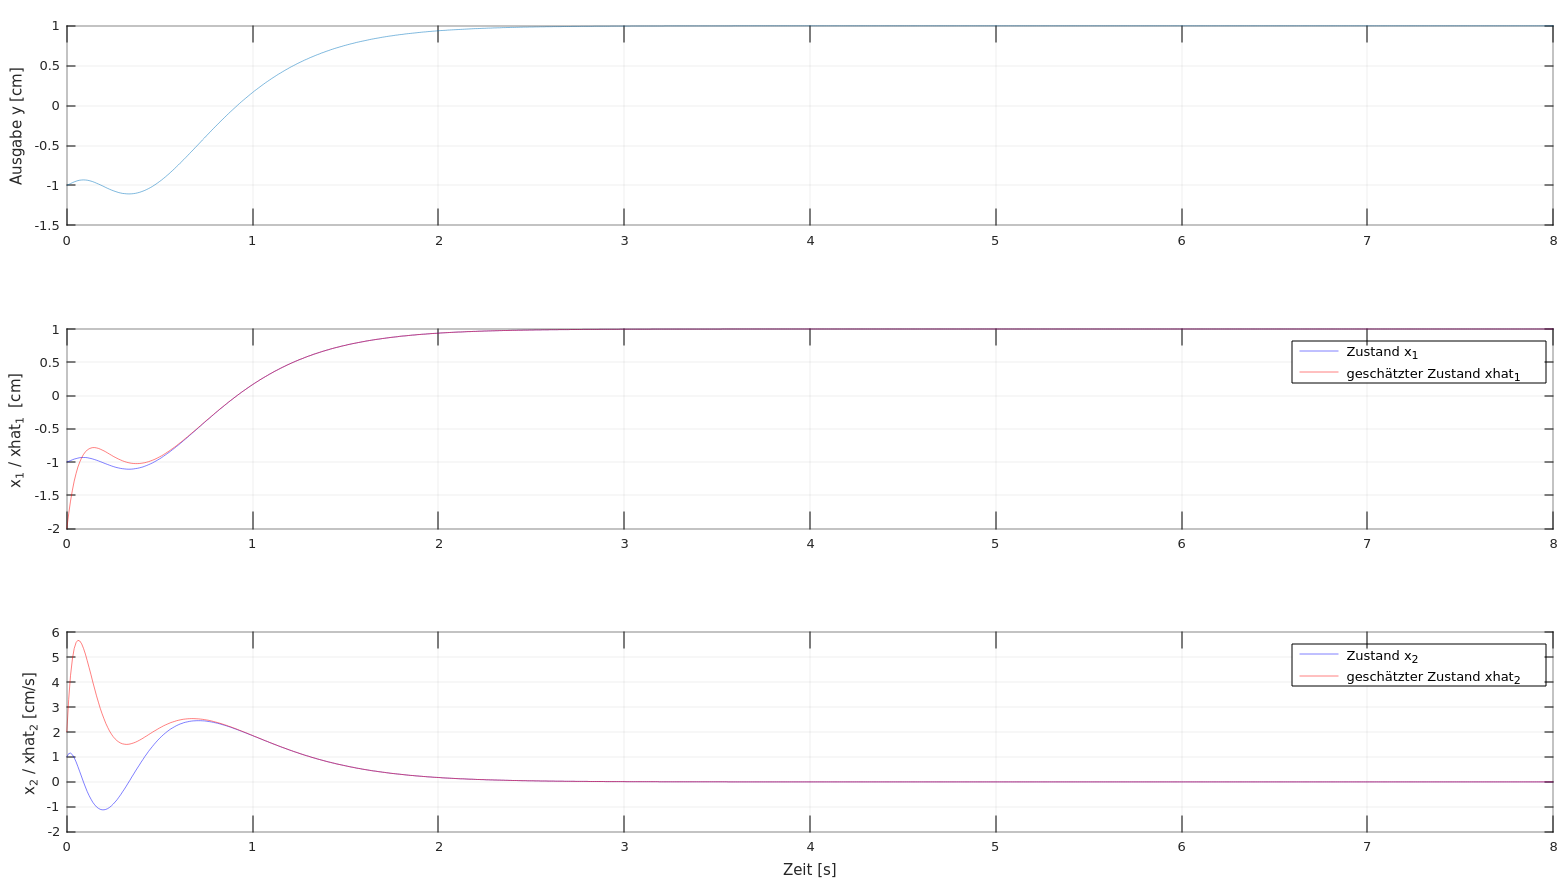
\includegraphics[width=\textwidth]{beobachterentwurfMitZustandsrueckfuehrung.png}
\captionsetup{labelformat=empty}
\caption{Abb. 8-2.1: Sprungantwort.}
\end{figure}

\section*{Aufgabe 8-3. Beobachterentwurf für das Pendel am Wagen (5 Punkte)}
\subsection*{a)}
\verb+[InvertedPendulumSimLuenbergerInit.m]+

\subsection*{b)}
\verb+[InvertedPendulumSimLuenberger.mdl]+\\

In Abbildung 8-3.1\footnote{Die Auflösung der Abbildungen ist hoch genug, um durch den PDF-Viewer ihrer Wahl eine angemessene Vergrößerung zu erreichen.} fällt zu aller erst auf, dass das System mit Rückführung der gemessenen Zustandsvariablen stabil ist. Das Pendel konnte in der instabilen Ruhelage gehalten werden.
Der geschätzte Zustand weicht stark vom gemessenen Zustand ab. Erst nach Drei bis Vier Sekunden stimmen diese überein und die Abweichung geht gegen Null. Am Ende der Swing-Up-Phase (Betrag des Pendelwinkels ist kleiner 1 rad) fällt auf, dass der Beobachterwert (exakt) mit der Wagenposition und der Wagengeschwindigkeit übereinstimmt. Die Pendelposition weicht nur noch ungefähr um $0.5$ rad ab.
\\

In Abbildung 8-3.2 konnte das System mit der Rückführung der beobachteten Zustandsvariablen nur durch "Zufall" stabilisiert werden. Das ist auch nicht verwunderlich, nachdem in Abbildung \mbox{8-3.1} bereits eine große Abweichung des beobachteten Zustands vom gemessenen Zustand festgestellt werden konnte. Die Beruhigungszeit beträgt mehr als 25s. Hier kann man nicht unbedingt von einem stabilen System sprechen.
Ab ungefähr 14 Sekunden verfällt das System in ein sich immer wiederholendes Muster. Das Pendel vollführt komplette Schwingungen um seinen Aufhängepunkt. Diese Schwingungen werden mit der Zeit immer langsamer. Bei Sekunde 21 ist bei der Pendelposition in Abbildung 8-3.2 dieses Langsamerwerden deutlich zu erkennen. Als Folge ist es dann möglich durch die langsamer gewordenen Schwingung das Pendel in der instabilen Ruhelage zu halten.

\begin{figure}[H]
\centering
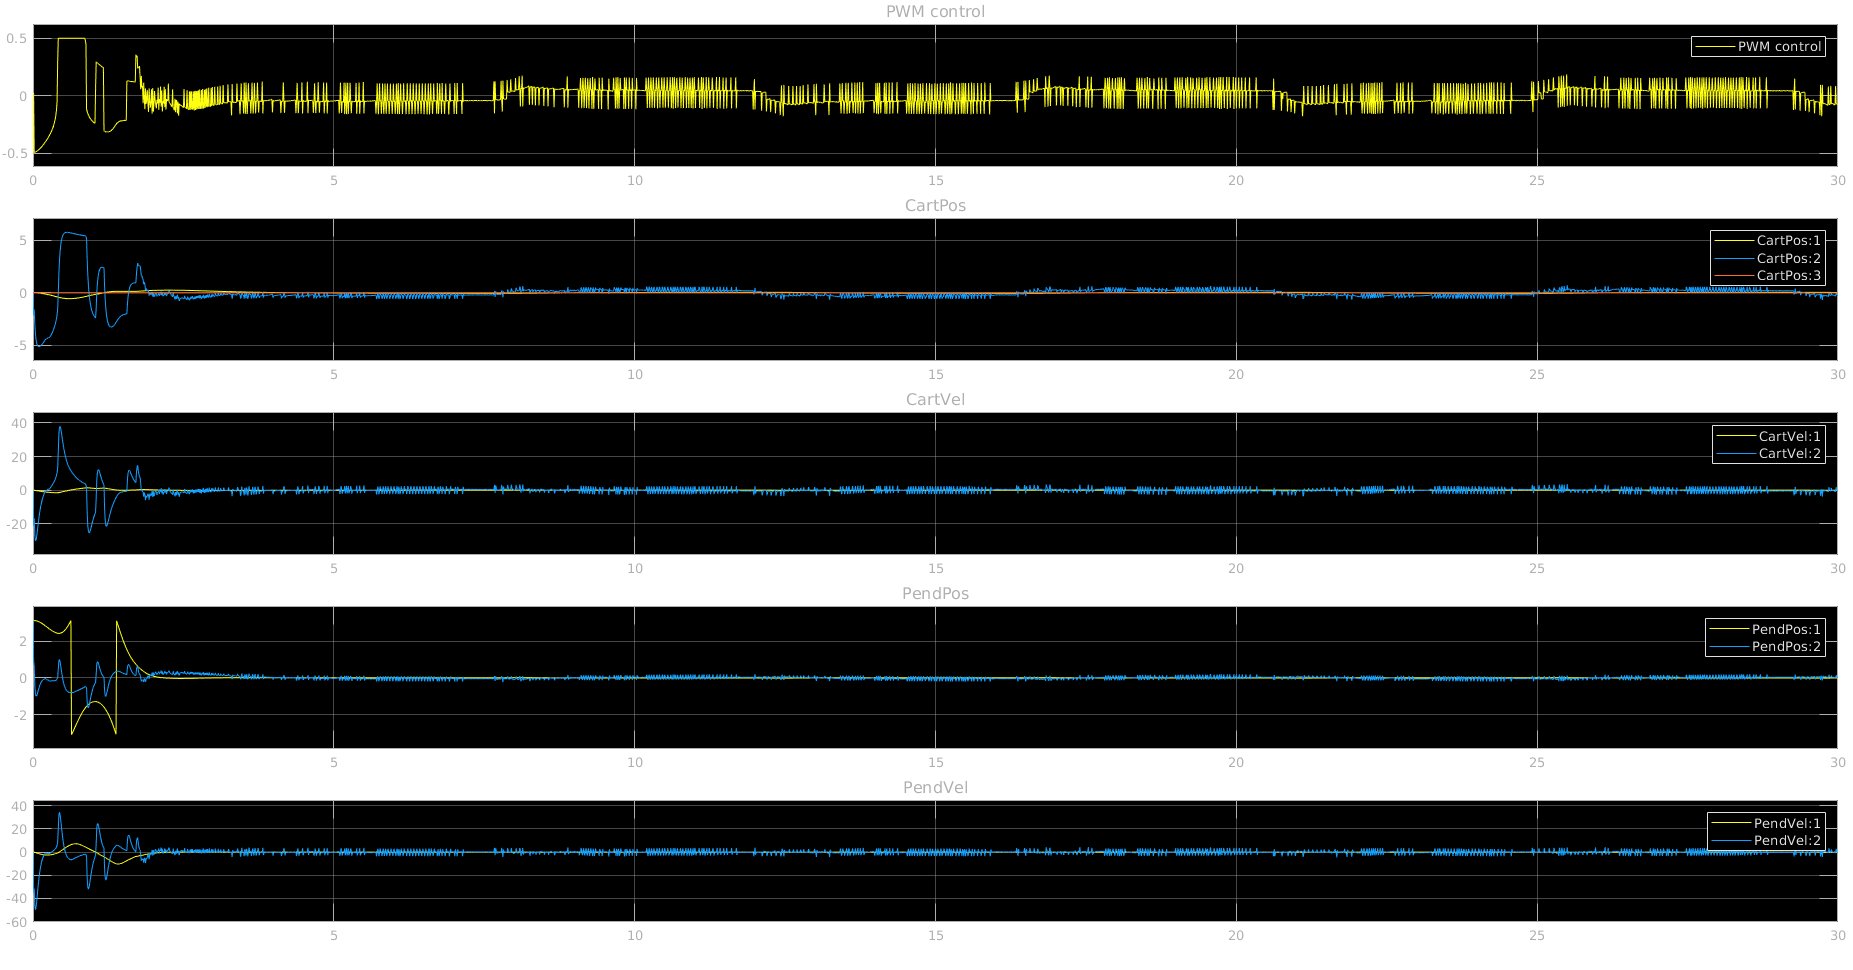
\includegraphics[width=\textwidth]{scope_measured_feedback.png}
\captionsetup{labelformat=empty}
\caption{Abb. 8-3.1: Scope der Simulation mit Rückführung der \textbf{gemessenen} Zustandsgrößen. Eigenwerte des Beobachters wurden doppelt so groß gewählt. Die gemessenen Werte sind gelb und die beobachteten Werte blau dargestellt.}
\end{figure}

\begin{figure}[H]
\centering
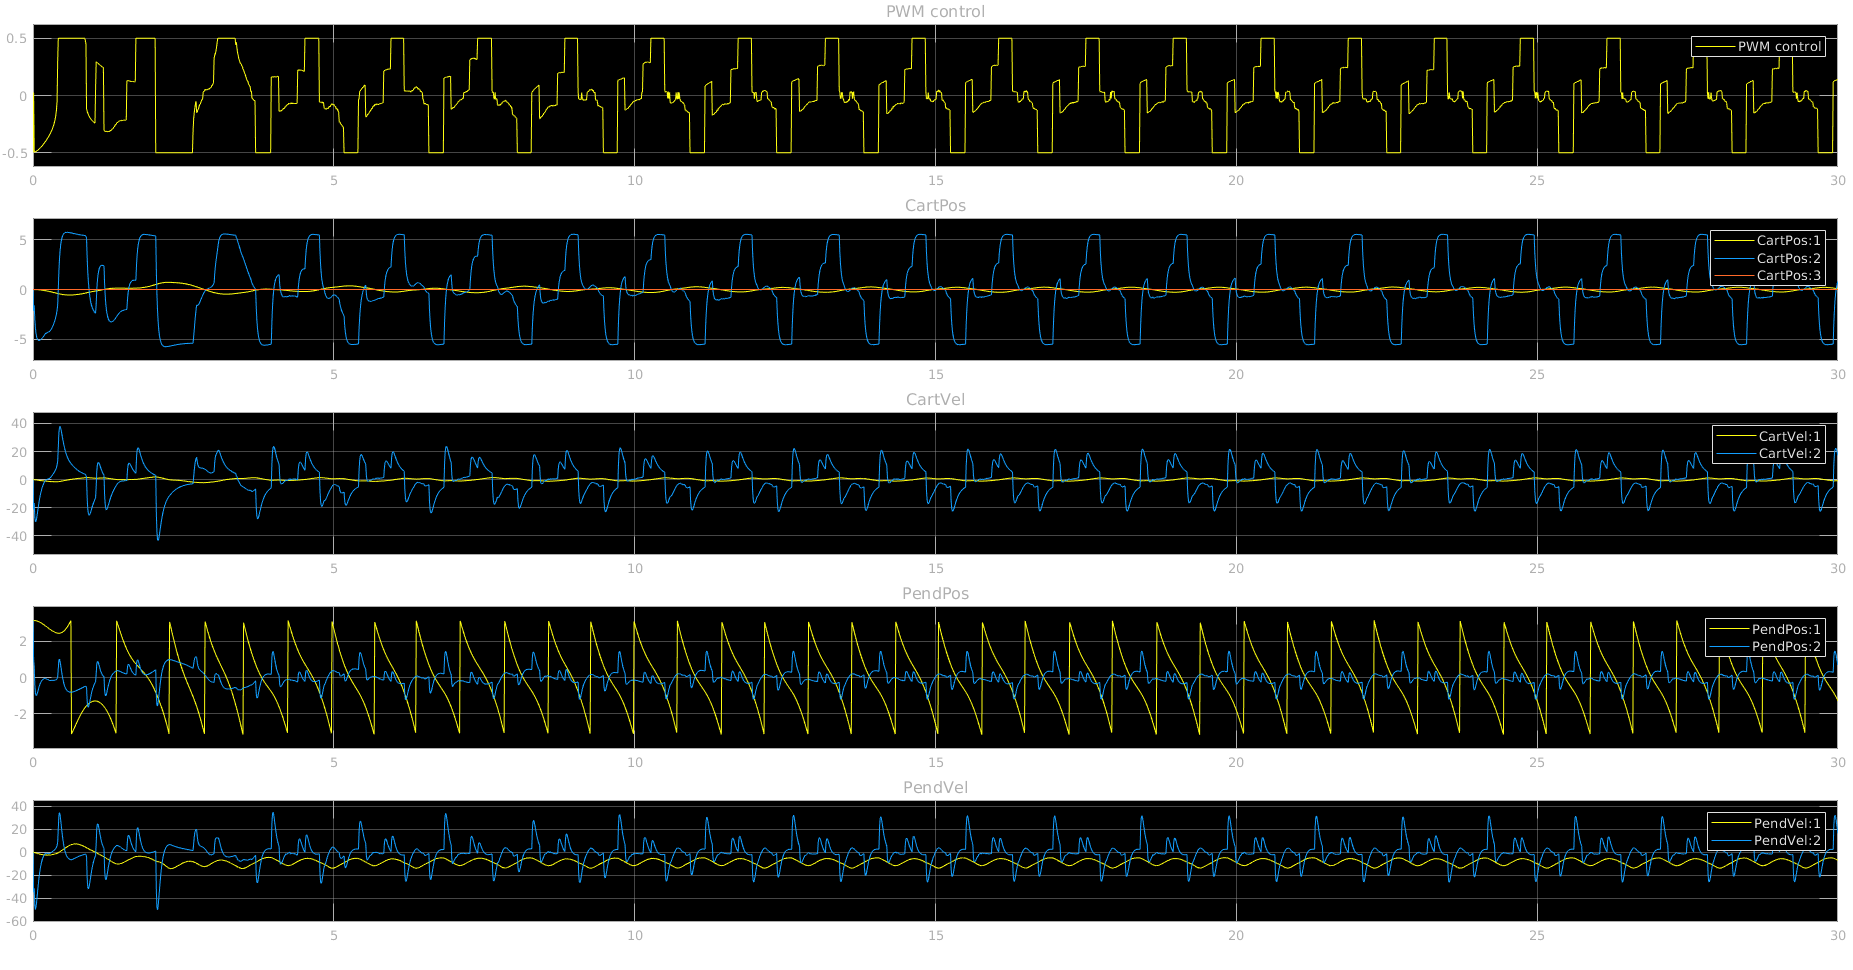
\includegraphics[width=\textwidth]{scope_observed_feedback.png}
\captionsetup{labelformat=empty}
\caption{Abb. 8-3.2: Scope der Simulation mit Rückführung der \textbf{beobachteten} Zustandsgrößen. Eigenwerte des Beobachters wurden doppelt so groß gewählt. Die gemessenen Werte sind gelb und die beobachteten Werte blau dargestellt.}
\end{figure}

\subsection*{c)}
In Abbildung 8-3.3 ist zu erkennen, dass das System nun stabil ist. Das Pendel wird in der instabilen Ruhelage gehalten obwohl die Schätzung teils sehr ungenau ist. Diese Ungenauigkeiten treten aber immer nur sehr kurz auf, sodass das System wenig bis gar nicht darauf reagiert bzw. reagieren kann. Solche extremen Abweichung sind beispielsweise ungefähr bei Sekunde 1 zu sehen. Die Schätzung der Wagenposition hat eine Spike (mehr als doppelt so groß wie gemessen) in negativer Richtung. Dasselbe passiert bei Wagengeschwindigkeit (nicht verwunderlich, da dies die Ableitung der Position ist). Für die Pendelposition ist dies auf der Abbildung nur schwer zu erkennen, aber ebenfalls bei ungefähr Sekunde 1 hat die Pendelgeschwindigkeit einen Spike in positiver Richtung, d.h. die Pendelposition tut dies auch. Bei hinreichender Vergrößerung ist dies auch bei der Pendelposition zu erkennen.\\
Dann ungefähr ab Sekunde 2 stimmen gemessener Zustand und geschätzter Zustand überein und das Pendel steht stabil in der instabilen Ruhelage.

\begin{figure}[H]
\centering
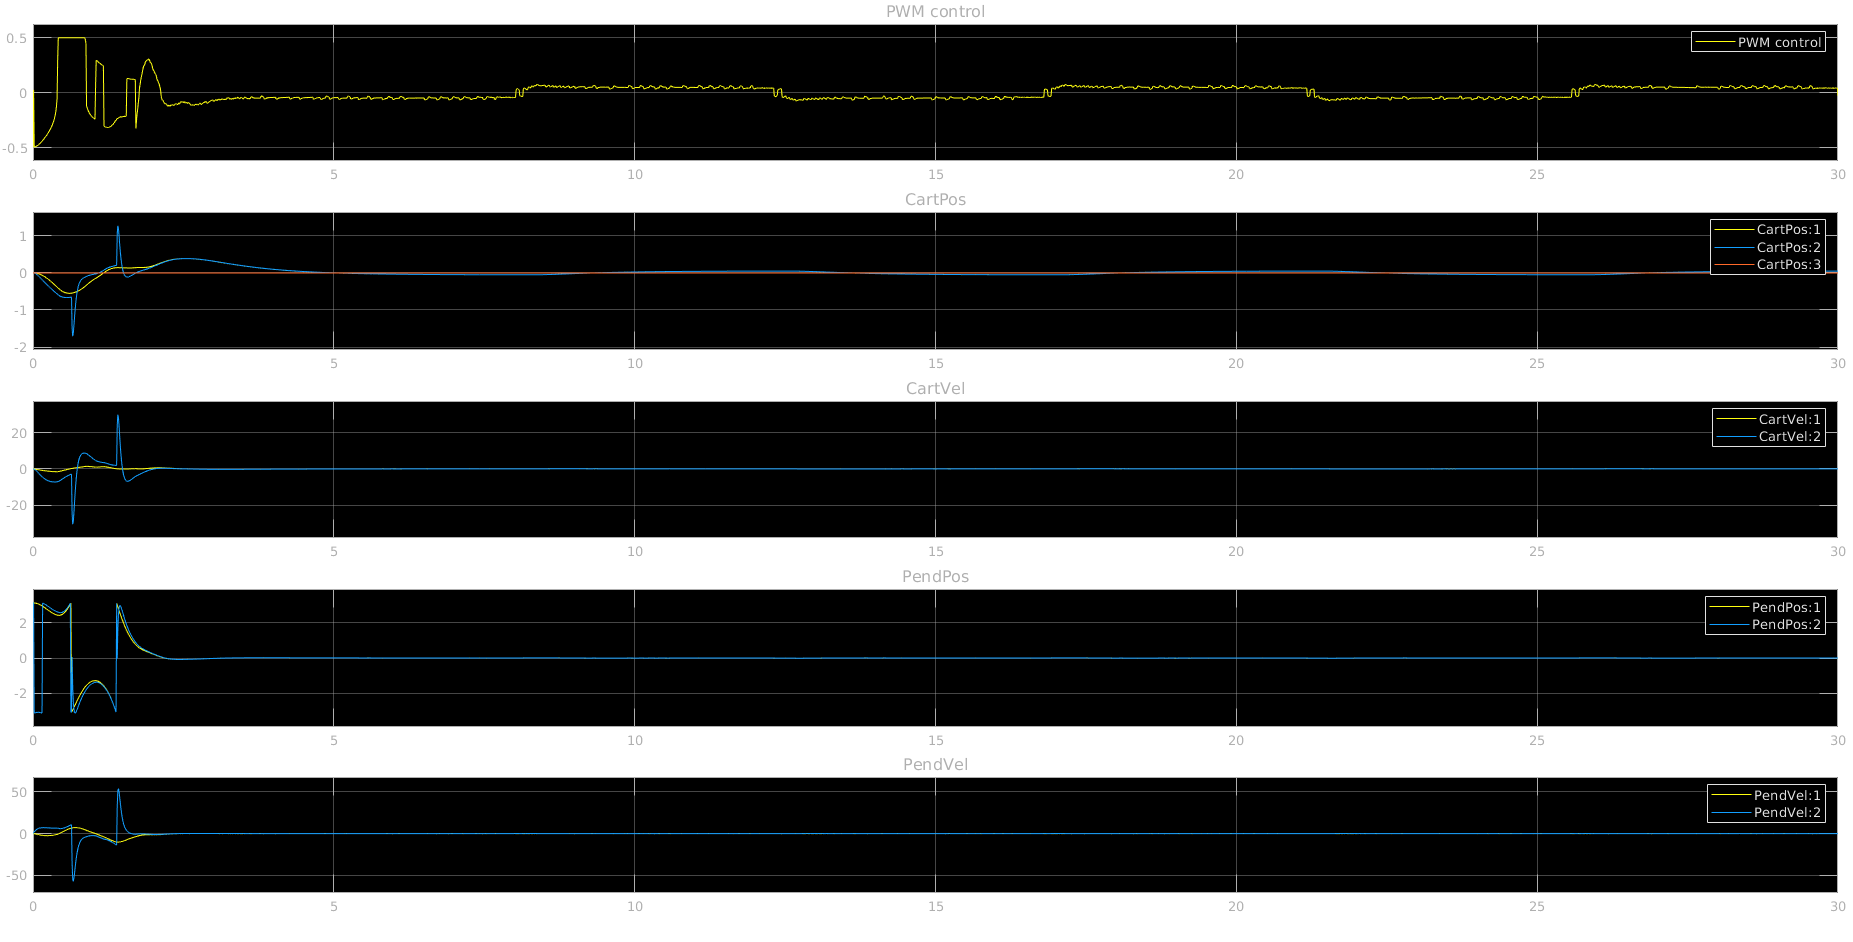
\includegraphics[width=\textwidth]{scope_observed_feedback_optimized.png}
\captionsetup{labelformat=empty}
\caption{Abb. 8-3.3: Scope der Simulation mit Rückführung der \textbf{beobachteten} Zustandsgrößen. Eigenwerte des Beobachters wurden sechsmal so groß gewählt. Die gemessenen Werte sind gelb und die beobachteten Werte blau dargestellt.}
\end{figure}

\subsection*{d)}

Die Simulation mit Rückführung der gemessenen Zustandsgrößen und hinzugefügten Störungen konnte mit Tiefpassfilter stabilisiert werden (Abbildung 8-3.4).\\
Die gemessenen und beobachteten Zustandsgrößen stimmen für die Wagenposition ungefähr ab Sekunde 2 überein. Davor gab es wie schon wie den Simulation zuvor (Abbildung 8-3.1 bis 8-3.3) kurze aber dafür sehr starke Abweichungen. Die beobachtete Pendelposition stimmt zu Anfang teilweise mit der gemessenen überein. Die Beobachtungswerte unterliegen hier großen Schwankungen.\\

Ohne Tiefpassfilter (Abbildung 8-3.5) gelang keine Stabilisierung.\\

In Abbildung 8.3-6 und 8.3-7 sind die Scopes der Simulation mit Rückführung der beobachteten Zustandsgrößen. Es gelang eine Stabilisierung in der instabilen Ruhephase. Es ist eindeutig zu erkennen, dass die abgeleiteten beobachteten Zustandsgrößen (Wagen- und Pendelgeschwindigkeit) nicht so stark von den Störungen beeinflusst werden wie die gemessenen. Bei den (direkt) beobachteten Zustandsgrößen (Wagen- und Pendelposition) ist dies schon deutlicher der Fall. Der Beobachter berücksichtigt die Störungen und kann diese rückführen, so dass das System stabil gehalten werden kann.


\begin{figure}[H]
\centering
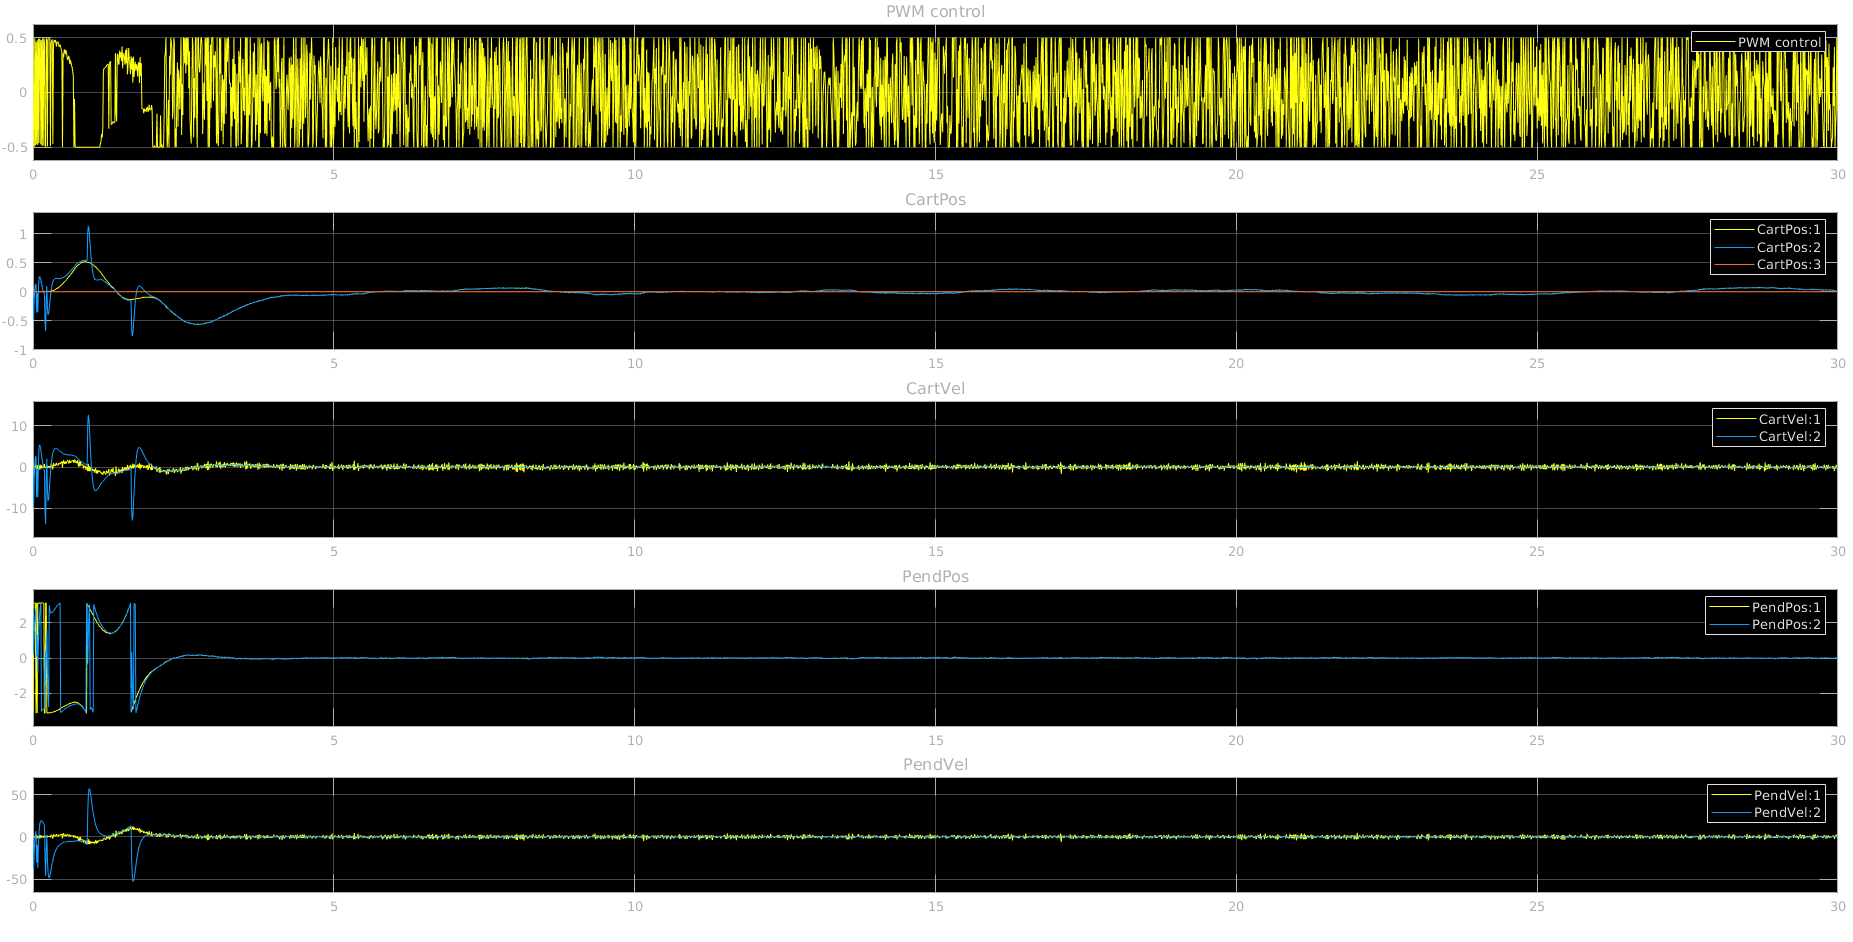
\includegraphics[width=\textwidth]{n1_scope_measured_noise_low_pass.png}
\captionsetup{labelformat=empty}
\caption{Abb. 8-3.4: Scope der Simulation mit Rückführung der \textbf{gemessenen} Zustandsgrößen. Eigenwerte des Beobachters wurden auf $\left[-45, -24, -21, -18\right]$ gewählt. Die gemessenen Werte sind gelb und die beobachteten Werte blau dargestellt. Der Simulation wurden Störungen hinzugefügt und es wurde ein Tiefpassfilter verwendet.}
\end{figure}
\begin{figure}[H]
\centering
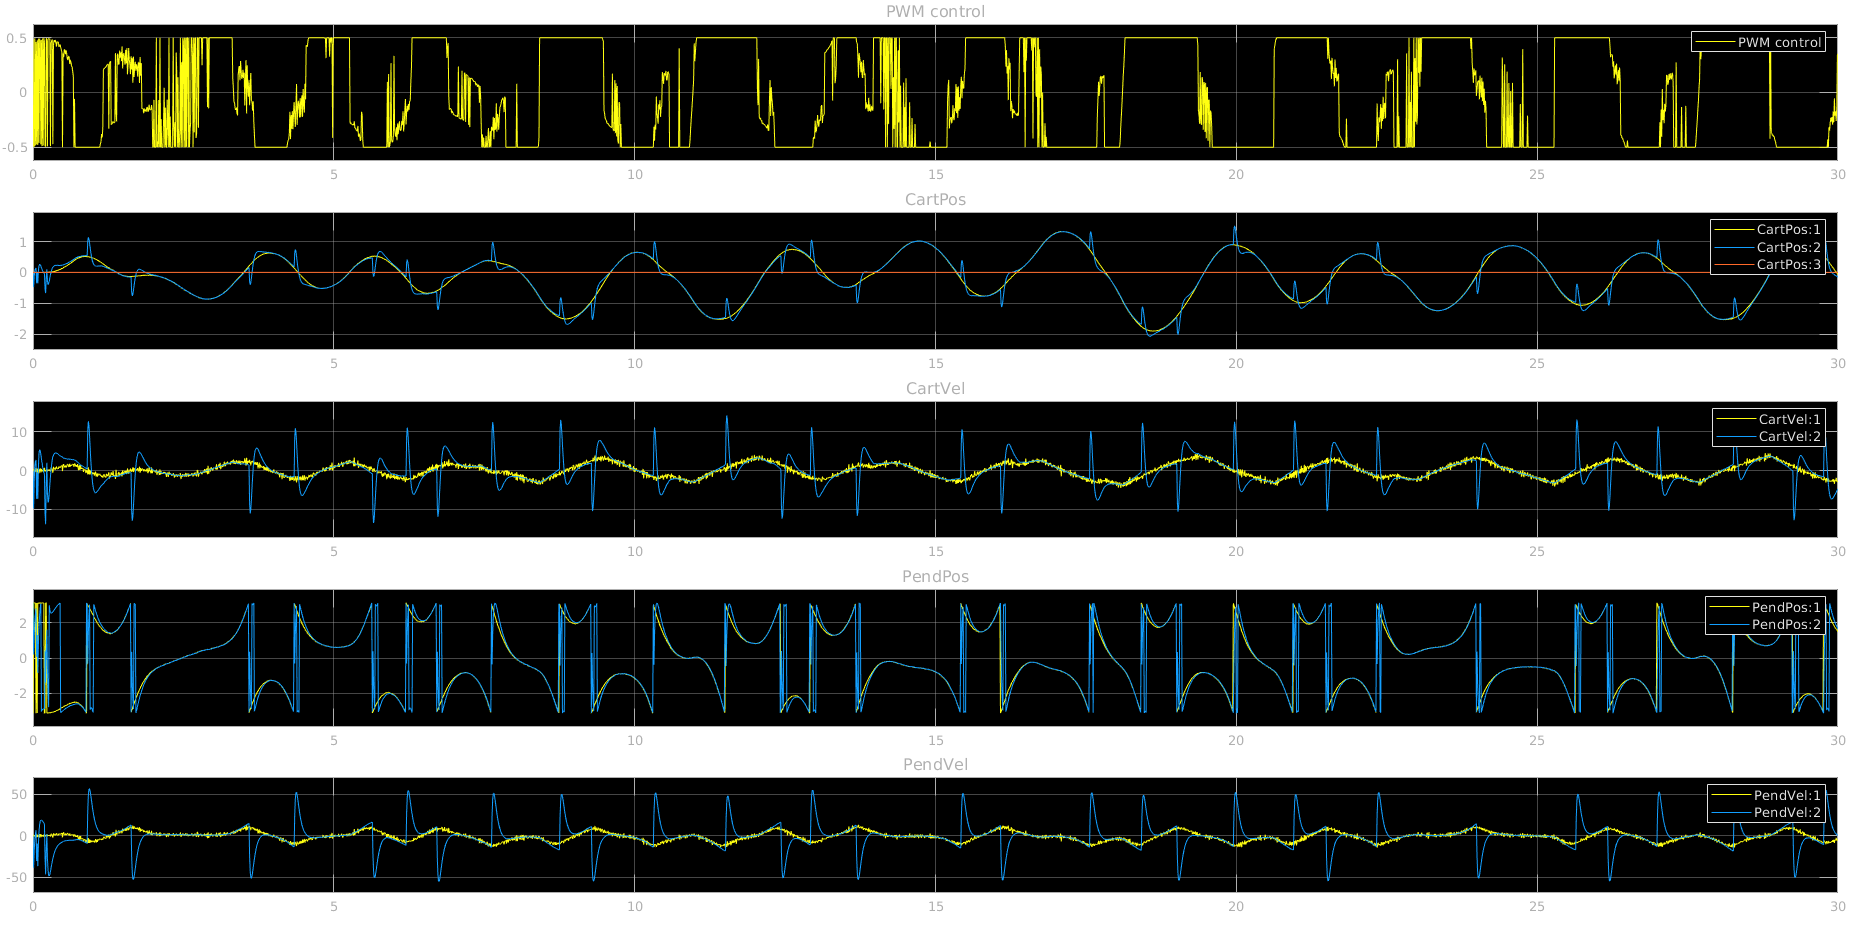
\includegraphics[width=\textwidth]{n2_scope_measured_noise.png}
\captionsetup{labelformat=empty}
\caption{Abb. 8-3.5: Scope der Simulation mit Rückführung der \textbf{gemessenen} Zustandsgrößen. Eigenwerte des Beobachters wurden auf $\left[-45, -24, -21, -18\right]$ gewählt. Die gemessenen Werte sind gelb und die beobachteten Werte blau dargestellt. Der Simulation wurden Störungen hinzugefügt und es wurde \textbf{kein} Tiefpassfilter verwendet.}
\end{figure}
\begin{figure}[H]
\centering
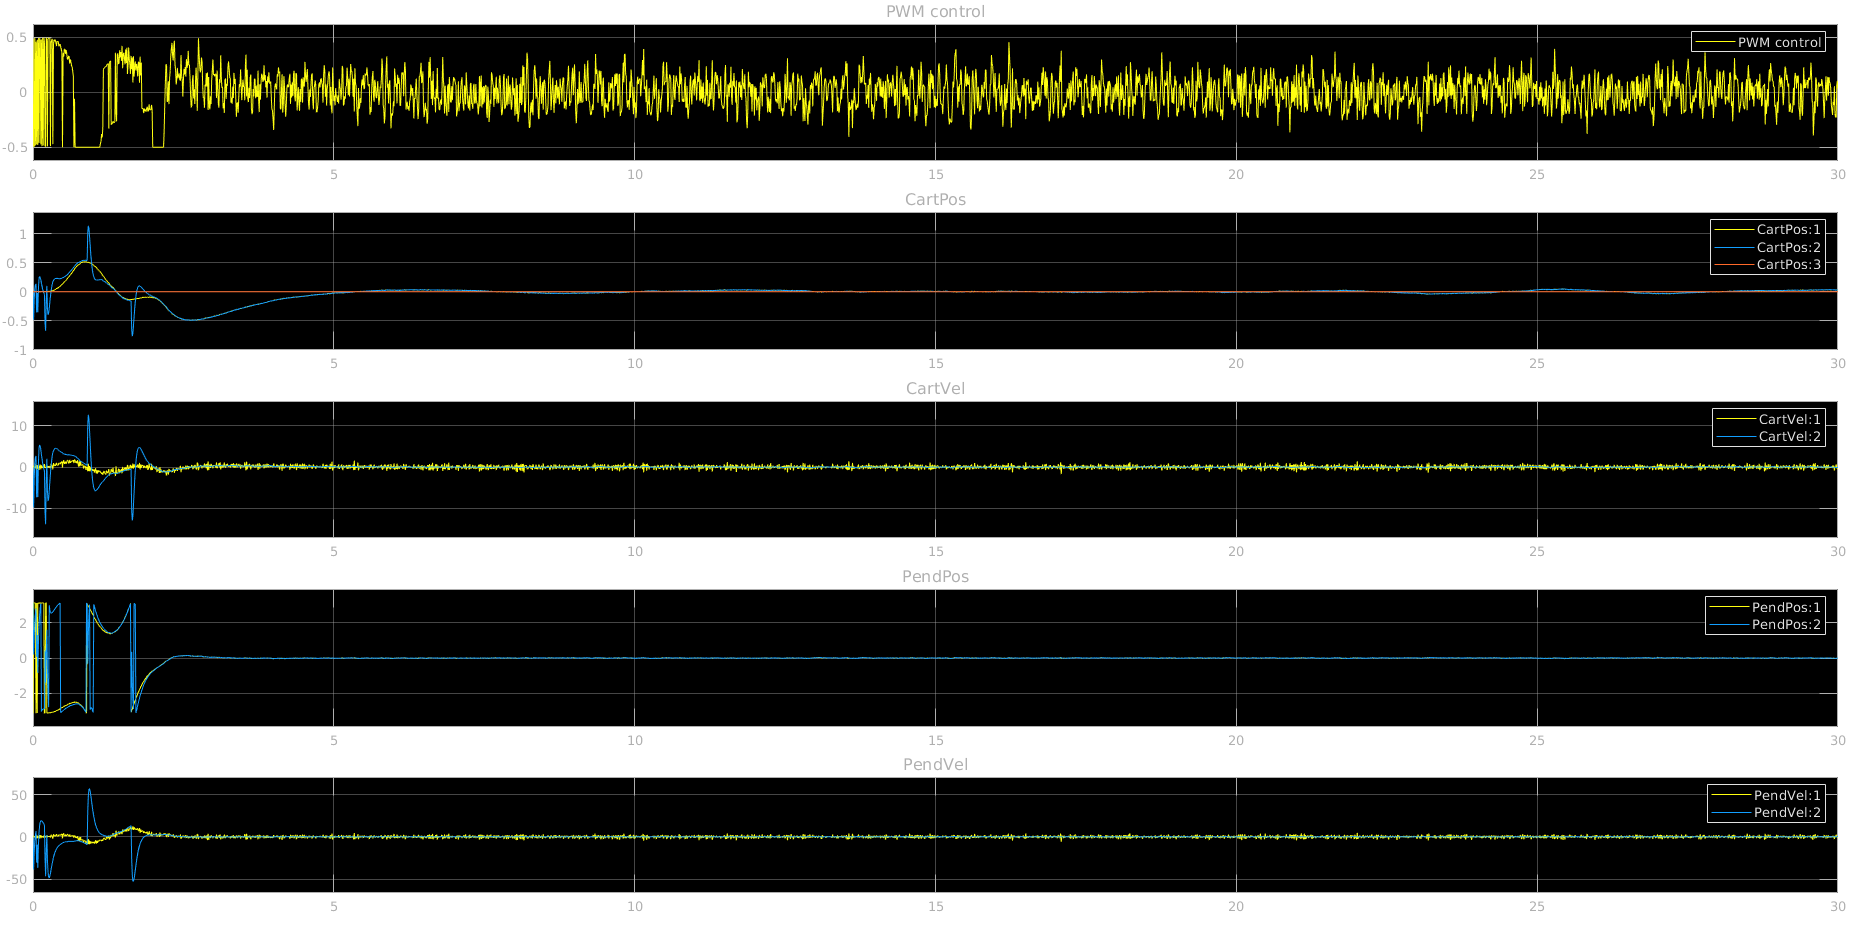
\includegraphics[width=\textwidth]{n3_scope_observed_noise.png}
\captionsetup{labelformat=empty}
\caption{Abb. 8-3.6: Scope der Simulation mit Rückführung der \textbf{beobachteten} Zustandsgrößen. Eigenwerte des Beobachters wurden auf $\left[-45, -24, -21, -18\right]$ gewählt. Die gemessenen Werte sind gelb und die beobachteten Werte blau dargestellt. Der Simulation wurden Störungen hinzugefügt und es wurde \textbf{kein} Tiefpassfilter verwendet.}
\end{figure}
\begin{figure}[H]
\centering
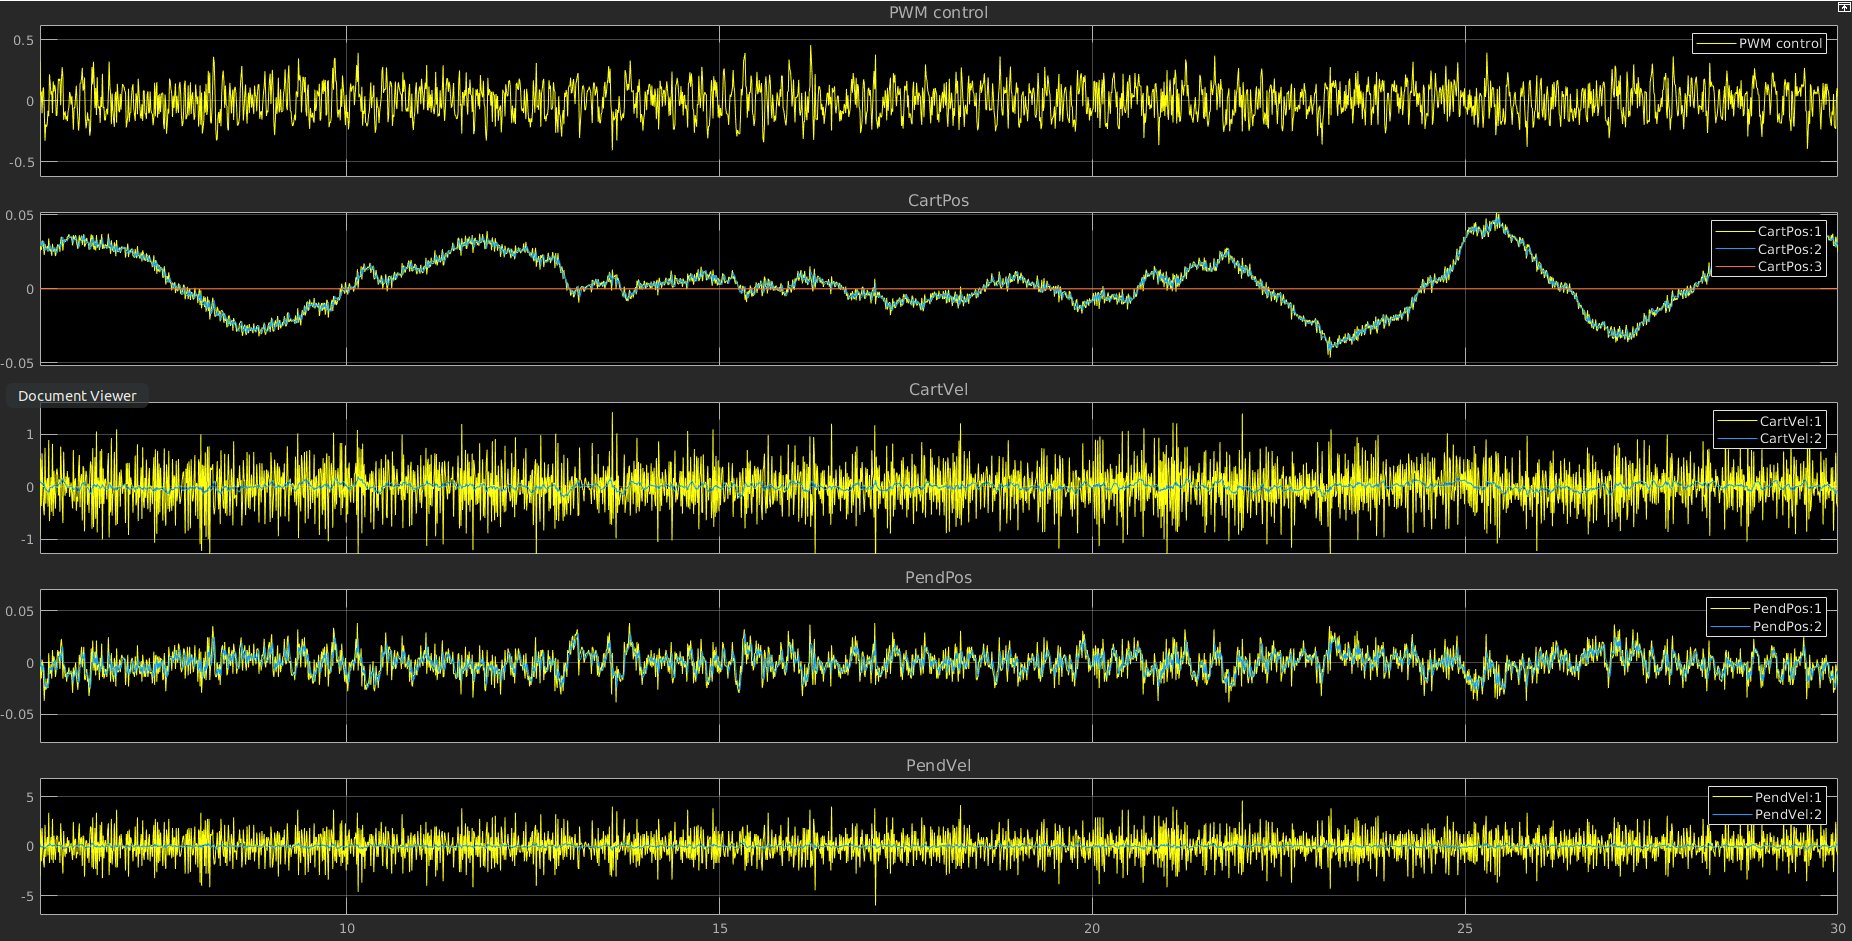
\includegraphics[width=\textwidth]{n3_scope_observed_noise_zoom.png}
\captionsetup{labelformat=empty}
\caption{Abb. 8-3.7: Starke Vergrößerung der instabilen Ruhephase von Abbildung 8-3.6.}
\end{figure}

\end{document}
